\documentclass{article}

\usepackage{../preamble}
\standalonetrue

\pagestyle{fancy}
\fancyhf{}
\rhead{Section \thesection}
\lhead{MATH 316 Review Session}
\rfoot{Page \thepage}


\title{MATH 316 Review Session}
\author{Ashtan Mistal}
\date{June 17 2021}

\begin{document}

\ifstandalone
\maketitle
\fi

\graphicspath{{./Lecture20/}}


\begin{itemize}
    \item The final exam is 2.5 hours long.
    \item The exam will \textbf{not} contain anything that wasn't covered during our lectures; Professor Pierce's notes covered extra material that will not be covered. 
\end{itemize}

Regarding the review session, please view the file uploaded to Canvas for the practice example we're doing. 

\section{Examples}

\subsection{Example 1: 2018 Final}

Laplace's equation in cylindrical coordinates. 

Consider the laplace's equation on a circular wedge with the following boundary contitions:

$$u_{rr} + \frac{1}{r} u_r + \frac{1}{r^2} u_{\theta \theta} = 0, \quad 0 \leq r \leq a \text{ and } 0 \leq r \leq \pi/4$$

$$u(r,0) = 1, \quad u_{\theta}(r, \frac{\pi}{4}) = 0, \quad u(a, \theta) = \sin(2 \theta) + 1$$

\begin{center}
    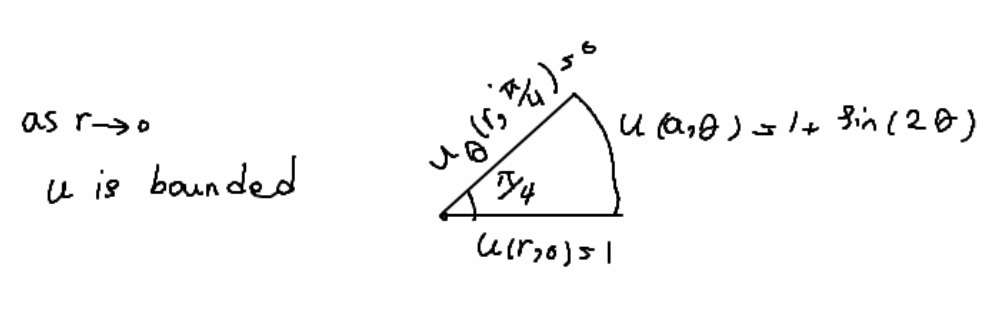
\includegraphics[width = 0.7 \textwidth]{1.png}
\end{center}

$$u(r, \theta) = w(\theta) + v(r, \theta)$$

$$w(\theta) = A \theta + B$$

$$w(0) = 1, \quad w_{\theta} (\frac{\pi}{4}) = 0 \Rightarrow w(\theta) = 1$$

Now, for $v(r, \theta)$:

$$\Delta v = 0$$

\begin{center}
    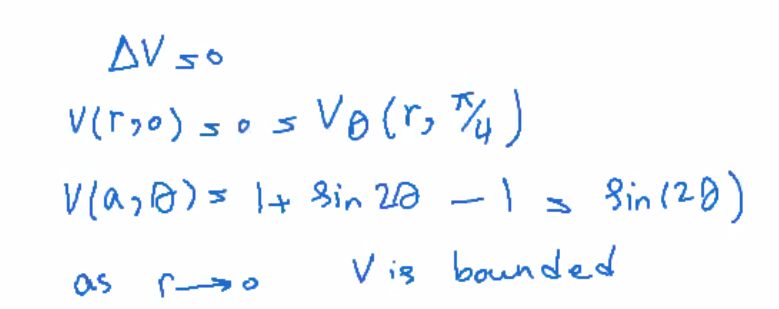
\includegraphics[width = 0.7 \textwidth]{2.png}
\end{center}

Using separation of variables, we get the following:

$$- \frac{r^2 R'' + r R'}{R} = \frac{\Theta''}{\Theta} = - \lambda$$

$\Theta$ function: $\Theta'' + \lambda \Theta = 0$. Using the factn that $\Theta(0) = 0 = \Theta'(\frac{\pi}{4})$, we get an eigenfunction of $\Theta_n = \sin( \mu_n \theta)$ for an eigenvalue of $\mu_n = \frac{(2n-1) \pi}{2 \frac{\pi}{4}} = 2(2n-1)$ for $n \in \NN$. This therefore makes $\lambda_n = 4 (2n-1)^2$. 

For the $R$ function, we have $r^2 R_n'' + r R_n' - \mu_n^2 R_n = 0$. This is a Cauchy-Euler equation. Therefore we guess a solution of $R_n(r) = r^{\alpha} \longrightarrow r^\alpha \left[ \alpha^2 - \alpha + \alpha - \mu_n^2 \right] = 0 \Rightarrow \alpha = \mu_n$

$$R_n(r) = A_n r^{\mu_n} + B_n r^{-\mu_n}$$

Since $u$ is bounded (therefore $v$ is bounded) as $ r \to \infty \Rightarrow B_n = 0$. 

Therefore, $v(r, \theta) = \sum_{n=1}^\infty A_n r^{\mu_n} \sin(\mu_n \theta)$. Substituting in BC: $v(a, \theta) = \sin (2 \theta) = \sum_{n=1}^\infty A_n a^{\mu_n} \sin(\mu_n \theta)$ with $\mu_n = 4n-2$. Because $4n-1 = 2$, $n = 1$. hence, $A_1 a^2 = 1 \rightarrow A_1 = \frac{1}{a_1}$ and $A_{n \neq 1} = 0$

$$\Rightarrow v(r, \theta) = \frac{r^2}{a^2} \sin(2 \theta)$$

Finally, we get the following as the final solution:

$$u(r, \theta) = 1 + \left( \frac{r}{a} \right)^2 \sin(2 \theta)$$

part (b) is asking us to sketch the solution at $theta = \frac{\pi}{4}$: $v(r, \frac{\pi}{4}) = \left( \frac{r}{a} \right)^2 \rightarrow u(r, 
\frac{\pi}{4}) = 1 + \left( \frac{r}{a} \right)^2$

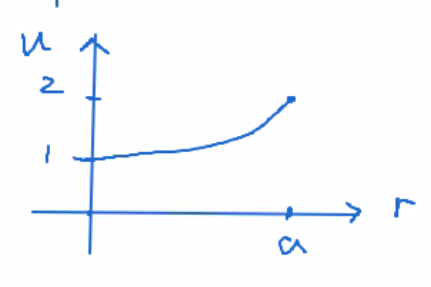
\includegraphics[width = 0.5 \textwidth]{3.png}

At $r = \frac{a}{2} \longrightarrow u(\frac{a}{2}, \theta) = 1 + \frac{1}{4} \sin(2 \theta)$

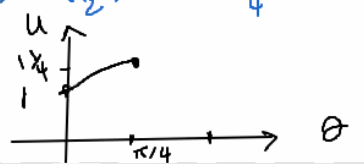
\includegraphics[width = 0.5 \textwidth]{6.png}

\subsection{Example 2 - December 2017 Final}

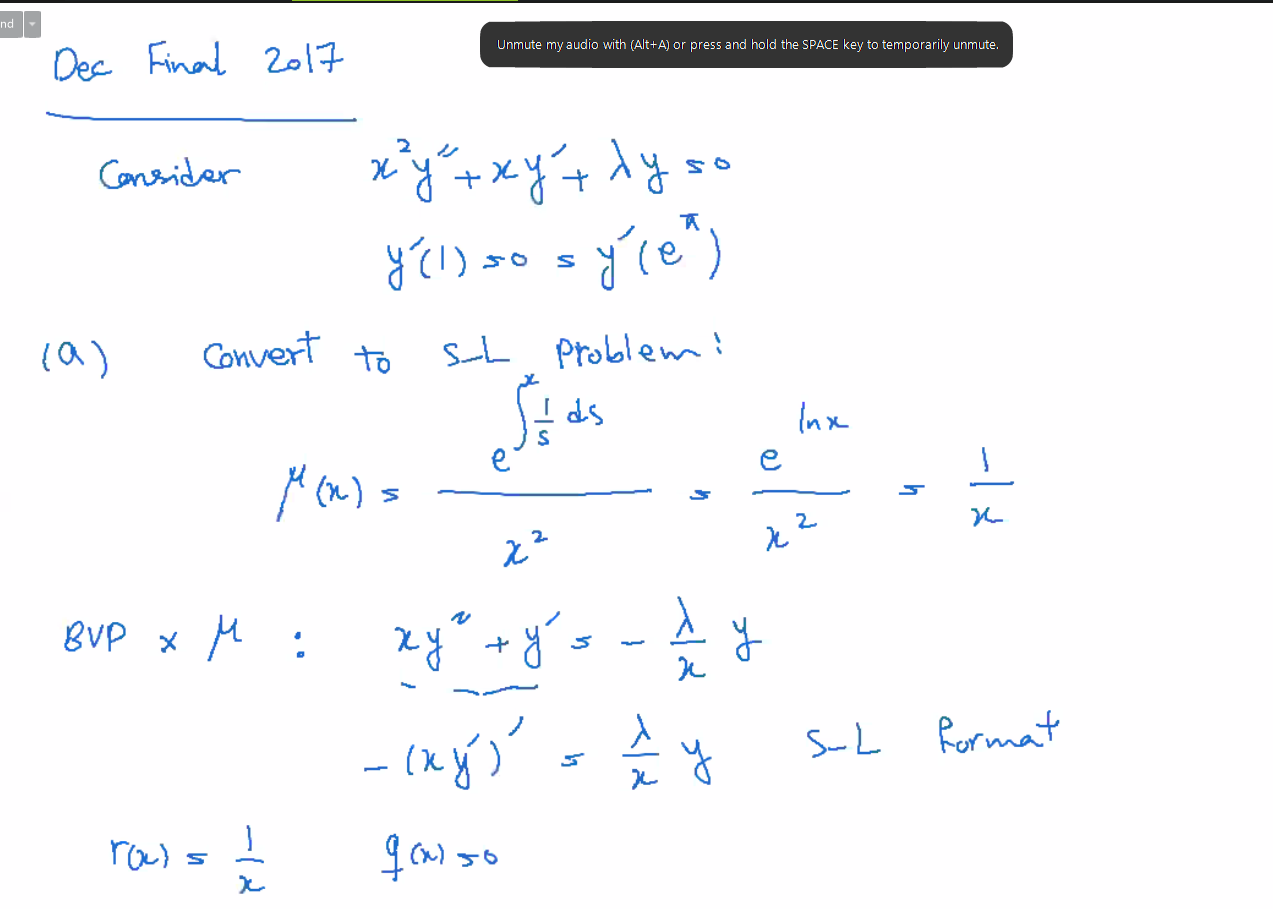
\includegraphics[width = 0.95 \textwidth]{4.png}

Solution: It's Cauchy - Euler equation guess solution is $y(x) = x^\alpha$. hence, $y'(x) = \alpha x^{\alpha - 1}$ and $y''(x) = \alpha (\alpha - 1) x^{\alpha - 2}$

Substitute this into the ODE:

$$\alpha (\alpha - 1) x^\alpha + \alpha x^{\alpha} + \lambda x^{\alpha} = 0$$

$$\alpha^2 - \alpha + \alpha + \lambda = 0 \Rightarrow \alpha^2 = - \lambda$$

According to theorem 5.1:1, if $q(x) \leq 0$ and $\alpha_1, \alpha_2, \beta_1, \beta_2 > 0$, then $\lambda_n \geq 0$. 

$y'(1) = 0 \longrightarrow \alpha_2 = -1$

$y'(e^\pi) = 0 \longrightarrow \beta_2 = 1$

Therefore, $\lambda_n$ could be negative. 

\hfill

Case 1: $\lambda = \mu^2 > 0$. Therefore $\alpha^2 = - \mu^2$. hence, $\alpha = \pm i \mu = e^{\pm i \mu \ln(x)}$

Therefore we have the following:

$$y(x) = A \cos(\mu \ln x) + B \sin(\mu \ln x)$$

$$y'(x) = - \frac{A \mu}{x} \sin(\mu \ln x) + \frac{B \mu}{x} \cos(\mu \ln x)$$

$$y'(1) = 0 \longrightarrow B = 0$$

$$y'(\pi) = 0 \longrightarrow - \frac{A \mu}{e^\pi} \sin(\mu \ln(e^\pi)) = 0 \Rightarrow \mu \pi = n \pi \therefore \mu_n = n \text{ for }n \in \NN$$

\hfill

Case 2: $\lambda = - \mu^2 < 0$. Therefore $\alpha = \pm \mu$

$$y(x) = A \cosh(\mu \ln(x)) + B \sinh (\mu \ln(x))$$

$$y'(x) = - \frac{A \mu}{x} \sinh(\mu \ln x) + \frac{B \mu}{x} \cosh(\mu \ln x)$$

$$y'(1) = 0 \longrightarrow B  =0$$

$$y'(e^\pi) = 0 \longrightarrow \frac{A \mu}{e^\pi} \sinh( \mu \ln(e^\pi)) = 0 \therefore A = 0$$

Hence this is a trivial solution. 

\hfill

Case 3: $\lambda = 0, \quad \alpha = 0$ (repeated roots)

$$y(x) = Ax + B \ln(x)$$

$$y'(x) = \frac{B}{x}$$

$$y'(1) = 0 \longrightarrow B = 0$$

$$y'(e^\pi) = 0 \longrightarrow B = 0$$

Hence, A is arbitrary. 

Therefore: $\lambda_0 = 0$ and $y_0(x) = 1$ is the eigenvalues and eigenfunctions respectively.

Finally, the eigenvalues are $\{ 0, n^2 \}$ and the eigenfunctions are $\{1, \cos(n \ln(x)) \}$. 

\hfill

For part (b), $\Delta u = 0$, $1 < r < e^\pi$, $0 $

$u(r, 0) = 0$ $u(r, \pi) = f(r)$

$u_r(1, \theta) = 0$, $u_r(e^\pi, \theta) = 0$

\begin{center}
    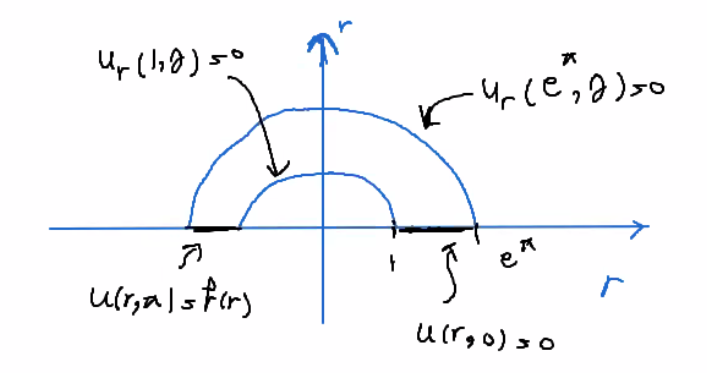
\includegraphics[width = 0.7 \textwidth]{7.png}
\end{center}

Solution: Here, we use separation of variables. 

$$- \frac{r^2 R'' + r R'}{R} = \frac{\Theta''}{\Theta} = \lambda$$

For the R function:

$$r^2 R'' + r R' + \lambda R = 0, \quad R'(1) = 0 = R'(e^\pi)$$

From part (a), $\lambda_0 = 0 \to R_0 = 1$, $\lambda_n = n^2 \to R_n = \cos(n \ln r)$ for $n \in \NN$

$\Theta$ function: $\Theta'' - \lambda \Theta = 0$.

$\lambda_0 = 0 \to \Theta_0 = A_0 \Theta + B_0$

$\Theta_0(0) = 0 \to B_0 = 0$

Therefore, $\Theta_0 = A_0 \Theta$

\hfill

$$\lambda_n = n^2: \quad \Theta_n'' - n^2 \Theta_n = 0 \to \Theta_n = A_n \cosh (n \theta) + B_n \sinh(n \theta)$$

$$\Theta_0(0) = 0 \to A_n = 0$$

As a result, $u(r, \theta) = A_0 \Theta + \sum_{n=1}^\infty B_n \sinh(n \theta) \cos(n \ln r)$

\begin{equation}
\label{star}
    u(r, \pi) = f(r) = A_0 \pi + \sum_{n=1}^\infty \underbrace{B_n \sinh(n \pi)}_{C_n} \cos(n \ln r)
\end{equation}

Using orthogonality relations:

Eigenfunctions: $R_0 = 1, R_n = \cos(n \ln r)$ and $r(x) = \frac{1}{r}$

(1): Multiply equation (\ref{star}) by $\frac{1}{r} \cdot 1$ and integrate:

$$\int_1^{e^\pi} \frac{1}{r} f(r) dr = \int_1^{r^\pi} \frac{1}{r} A_0 \pi dr + \sum_{n=1}^\infty C_n \int_1^{e^\pi} \frac{1}{r} \cos(n \ln r) dr$$

$$A_0 = \frac{\in_1^{e^\pi} \frac{1}{r} f(r) dr}{\pi \int_1^{e^\pi} \frac{dr}{r}} = \frac{\int_1^{e^\pi} \frac{1}{r} f(r) dr}{\pi \left( \left. \ln(r) \right|_1^{e^\pi} \right)} = \frac{\int_1^{e^\pi} \frac{1}{r} f(r) dr}{\pi^2}$$

(2): Multiply \ref{star} by $\frac{1}{r} \cos(m \ln r)$ and integrate:

$$\int_1^{e^\pi} \frac{1}{r} f(r) \cos(m \ln r) dr = A_0 \pi \int_1^{e^\pi} \frac{1}{r} \cos(m \ln r) dr + \sum_{n=1}^\infty C_n \int_1^{e^\pi} \frac{1}{r} \cos(m \ln r) \cos(n \ln r) dr$$


\begin{center}
    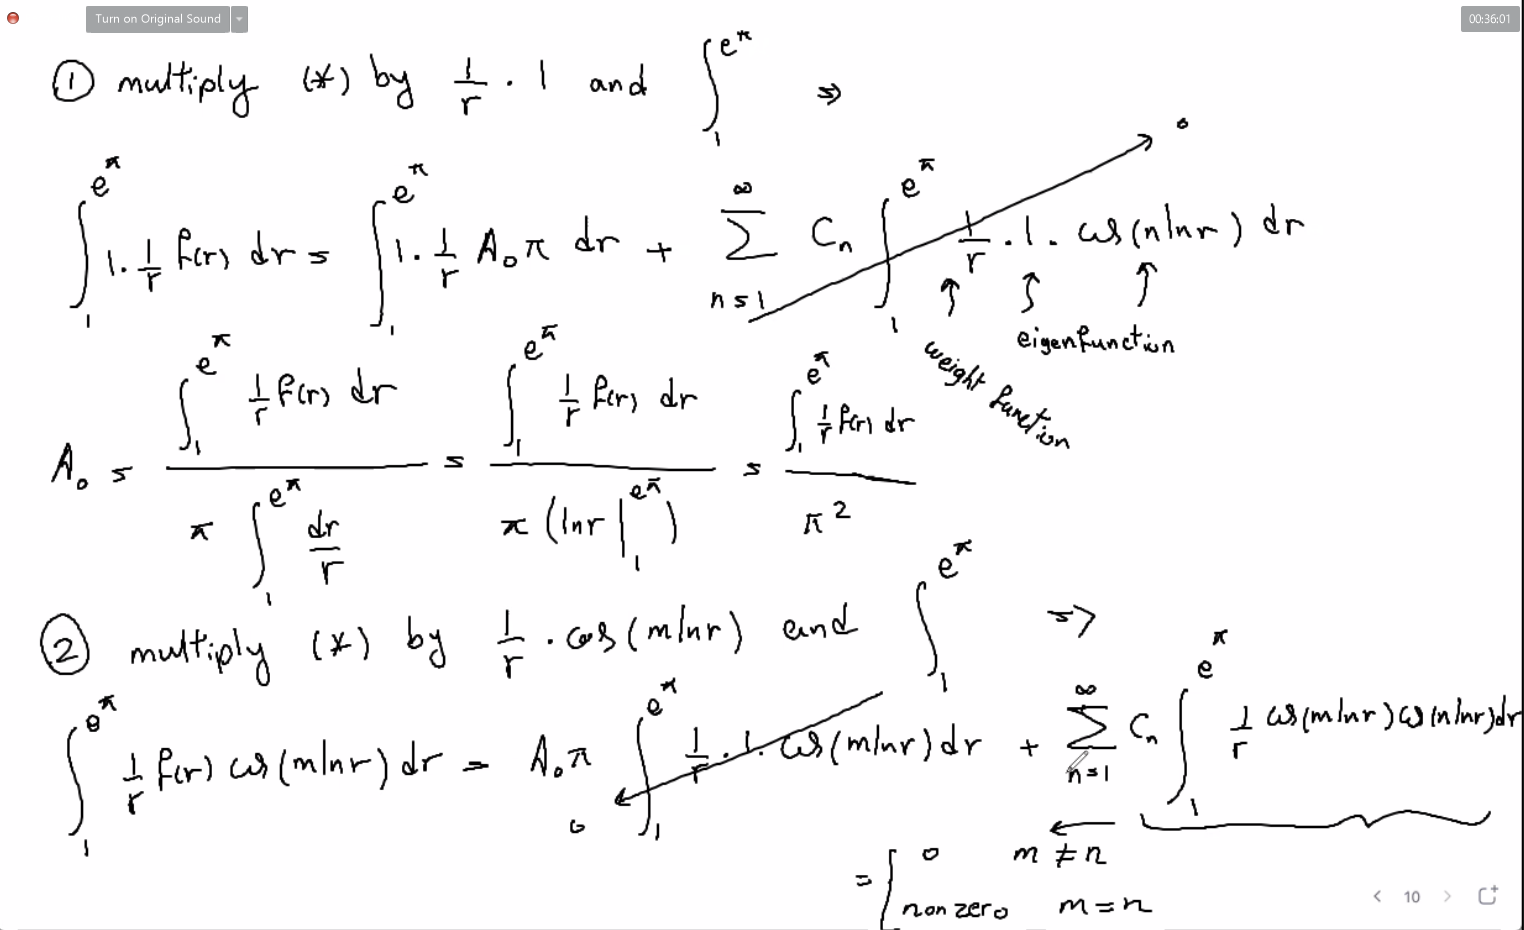
\includegraphics[width = 0.9 \textwidth]{8.png}
\end{center}

\begin{center}
    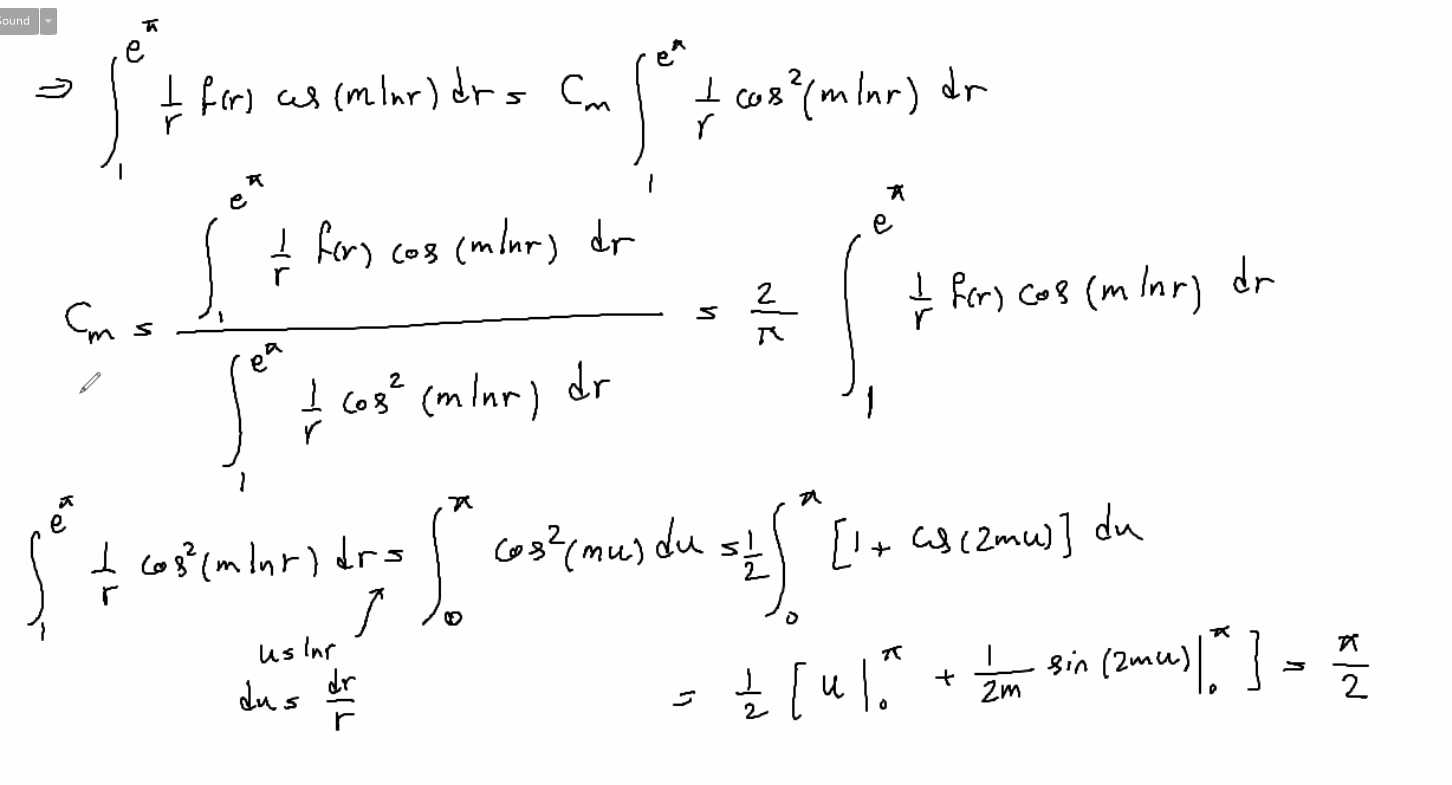
\includegraphics[width = 0.9 \textwidth]{10.png}
\end{center}

\begin{center}
    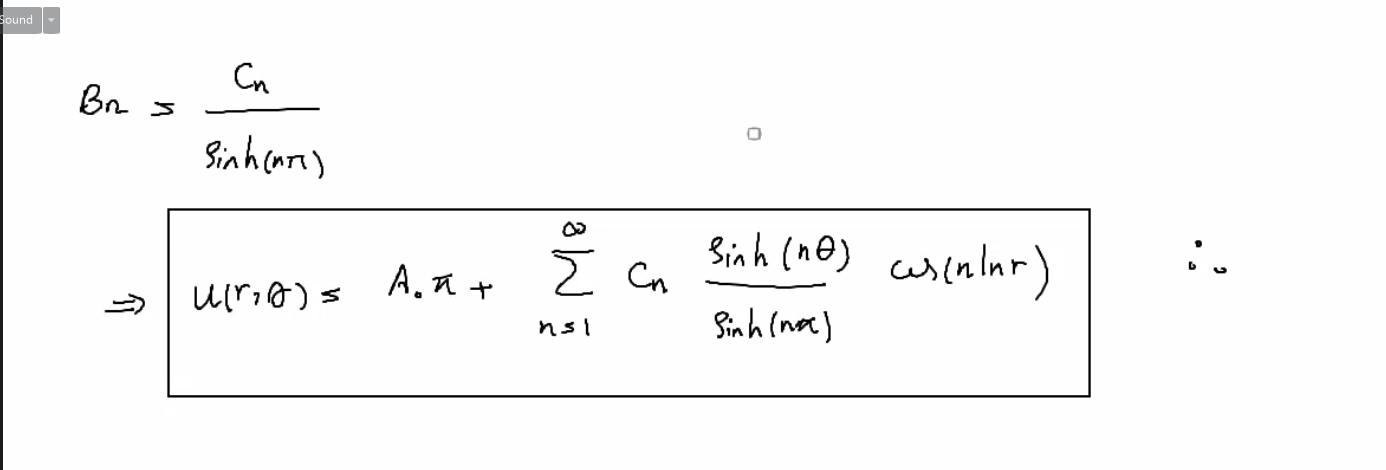
\includegraphics[width = 0.9 \textwidth]{11.png}
\end{center}

\section{Office Hours}

General Notes:

\begin{itemize}
    \item if we have Dirichlet boundary condition we do an odd extension, Neumann then even. 
\end{itemize}

\subsection{Final 2014}

Wave equation:

$$u_{tt} = u_{xx} - \gamma u, \quad 0 < x < 1, \quad t > 0$$
BC:
$$u(0,t) = u(1,t) = 0$$

IC:

$$u(x,0) = 0, \quad u_t(x,0) = g(x)$$

For part (a), we do the following:

$$u(x,t) = X(x) T(t) \rightarrow \frac{\ddot{T}}{T} + \gamma = \frac{X''}{X} = - \lambda$$

BVP:

$$X'' + \lambda X = 0$$

$$X(0) = 0 = X(1)$$

This is a P1 problem. 

Hence, $\lambda_n = \left( \frac{n \pi}{1} \right)^2$ and $X_n = \sin(n \pi x)$ for $n \in \NN$. 

\hfill

IVP:


$$\frac{\ddot{T}_n}{T_n} + \gamma = -(n \pi)^2 \Rightarrow \ddot{T}_n + \underbrace{(\gamma + (n \pi)^2 )}_{\mu_n^2} T_n = 0$$

$$T_n(t) = A_n \cos(\mu_n t) + B_n \sin(\mu_n t)$$

Substituting in the initial conditions:

$$u(x,0) = 0 \Rightarrow A_n = 0$$

$$\Rightarrow T_n = B_n \sin(\mu_n t)$$

$$u(x,t) = \sum_{n=1}^\infty B_n \sin(n \pi x) \sin(\mu_n t)$$

To find $B_n$, we use the second IC:

$$u_t(x,0) = g(x) = \sum_{n=1}^\infty B_n \mu_n \sin(n \pi x)$$

$$\Rightarrow B_n \mu_n = \frac{2}{1} \int_0^1 g(x) \sin(n \pi x) dx \rightarrow B_n = \frac{2}{\sqrt{\gamma + (n \pi)^2}} \int_0^1 g(x) \sin(n \pi x) dx$$

b) $\gamma = 7 \pi^2$ and $g(x) = \sin(3 \pi x)$

$$\sin(3 \pi x) = \sum_{n=1}^\infty B_n \mu_n \sin(n \pi x)$$

$n = 3$ and $B_3 \mu_3 = 1$ and $\mu_3 = \sqrt{7 \pi^2 + (3 \pi)^2} = 4 \pi$

Finally, $B_3 = \frac{1}{4 \pi}$

$$u(x,t) = \frac{1}{4 \pi} \sin(3 \pi x) \sin(4 \pi t)$$

\hfill

Sketch the solution for $t = \frac{3}{8} \Rightarrow u(x, \frac{3}{8}) = \frac{-1}{4 \pi} \sin(3 \pi x)$

\begin{center}
    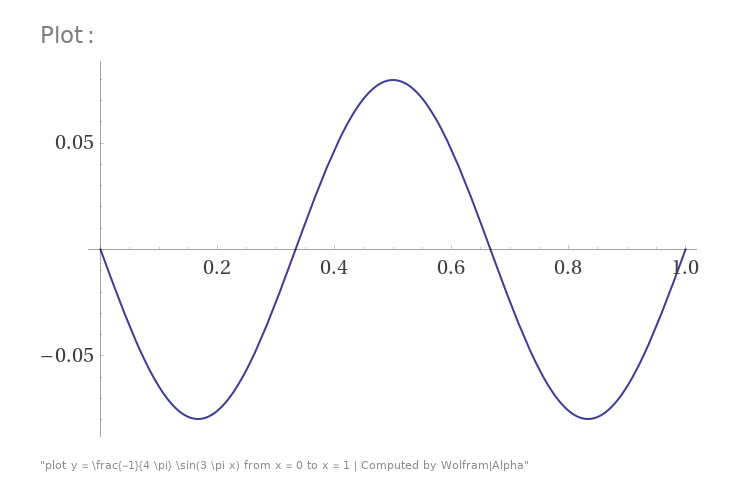
\includegraphics[width = 0.8 \textwidth]{12.png}
\end{center}













\end{document}